\documentclass[tikz,border=10pt]{standalone}
\usetikzlibrary{intersections}

\begin{document}
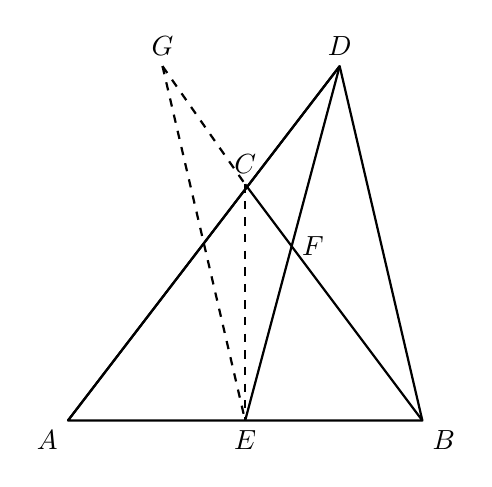
\begin{tikzpicture}[scale=1.5,thick,line join=round]

    % 1. 定义坐标 (基于视觉比例大致设定)
    \coordinate (A) at (0,0);
    \coordinate (B) at (3,0);
    \coordinate (E) at (1.5,0);
    \coordinate (D) at (2.3,3);
    \coordinate (C) at (1.5,2); % C 置于 AD 连线上
    \coordinate (G) at (0.8,3);   % 辅助顶点 G

    % 2. 绘制实线路径
    \draw (A) -- (B) -- (D) -- cycle; % 主三角形框
    \draw (A) -- (D);                % 线段 AD
    \draw (C) -- (B);                % 线段 CB
    \draw (E) -- (D);                % 线段 ED

    % 3. 绘制虚线路径
    \draw[dashed] (C) -- (E);
    \draw[dashed] (G) -- (E);
    \draw[dashed] (G) -- (C);

    % 4. 计算交点 F (BC 与 ED 的交点)
    \path[name path=BC] (B) -- (C);
    \path[name path=ED] (E) -- (D);
    \path [name intersections={of=BC and ED, by=F}];

    % 5. 标注点位
    \node[below left] at (A) {$A$};
    \node[below right] at (B) {$B$};
    \node[below] at (E) {$E$};
    \node[above] at (D) {$D$};
    \node[above] at (C) {$C$};
    \node[right] at (F) {$F$};
    \node[above] at (G) {$G$};

\end{tikzpicture}
\end{document}